\documentclass{article}[18pt]
\usepackage{../../../format}
\lhead{Sofware Engineering - Testing}


\begin{document}
\begin{center}
\underline{\huge A testing perspective}
\end{center}
\section{Why test software?}
Software is an ISP, so no definitive specification, many possible solutions and no definitive way of knowing how good a solution is. Hence we need to test a solution to see how well it fits. And we can regard the process of testing as being an ISP, needing a design approach.\\
\\
Alternate answer:
\begin{itemize}
	\item To discover problems (a developer-centric view): does the component/system behave as expected?
	\item To assess quality (a customer/market-led view): is the system acceptable to the end users?
	\item Plan driven forms of development tend to put early emphasis on the developer perspective, agile forms tend to emphasise both perspectives throughout.
\end{itemize}
\section{Limitations}
Because of the characteristics of an ISP, testing can't demonstrate that software is free of defects or that it will always behave as specified.\\
\\
In no sense does testing "prove" anything, it can only be a means of providing confidence about software
\section{Where's the challenge?}
\begin{itemize}
	\item Many people find designing tests offers an intellectual challenge, regardless of perspective
	\item In some ways it is a bit like a game, you are pitting your wits against the designer of the software
	\item The job of the tester is to "think outside of the box" and try to avoid making the same (possibly wrong) assumptions that the developer might have done
\end{itemize}
\section{Definitions}
\textbf{Error} - Mistakes made when designing (or coding), which may be of logic (using the wrong operator) or of interpretation (such as misunderstanding a requirement). Often terms bugs and not usually detectable by a compiler\\
\\
\textbf{Fault} - The result of an error (or its representation). Faults may be of commission(something that should be different, such as the wrong operator) or omission(something absent). The latter tend to be harder to detect and resolve\\
\\
\textbf{Failure} - Occurs when a fault executes (or doesn't in the case of omission). Might not occur immediately, the fault may seed a later system crash\\
\\
\textbf{Test} - Exercising software with test cases to check correctness or find faults\\
\\
\textbf{Test case} - A set of inputs together with the expected outputs
\section{The Test Oracle}
The key action when testing is to compare the value(s) or state changes that are output from our test case with some predicted value(s) or state changes.\\
\\
The predictions are produced by the test oracle, a mythical being that "knows all the answers"\\
\\
So designing test cases involves specifying both input and output values/states. For more complex stages, such as acceptance testing, the oracle may actually take the form of a set of expert users who "judge" whether or not the outputs are acceptable.
\section{Testing in the Life Cycle}
\begin{itemize}
	\item Testing is one of the activities that is organised quite differently within waterfall and agile development processes, although the actual test details may not be very different
	\item Development usually has a hierarchy of test activities corresponding with particular stages of development, regardless of how they are organised.
	\item With agile forms, testing may be more interpolated with development activities, depending on the form. In particular, with XP, there is the practice of writing the testes before writing the code
\end{itemize}
\begin{center}
	\includegraphics[scale=0.7]{"v model"}
\end{center}
\section{Regression Testing}
If we make changes to the elements of the system then we need to test everything again. This process is termed regression testing and is used to ensure that the changes have not destabilised code that previously worked
\section{Canary Release}
Even after all the testing, releasing a new version of software to users might reveal errors that the testing didn't uncover. One technique that can help here is to initially release it to selected users before making it publicly available.
\section{The two major test strategies}
\textbf{Functional testing} - Black box testing where we have no details of the inner workings of the parts of the system being tested. Helps to establish confidence\\
\\
\textbf{Structural testing} - White box/clear box testing, for which the implementation is visible and can be used to generate test cases
\section{Error and Fault taxonomies}
Not all errors are of equal importance in terms of their effect
\begin{itemize}
	\item A system may well be able to continue functioning in the presence of errors, although not fully correctly
	\item Some errors may only occur on very rare occasions
\end{itemize}
This is one example of a scale for severity:
\begin{center}
	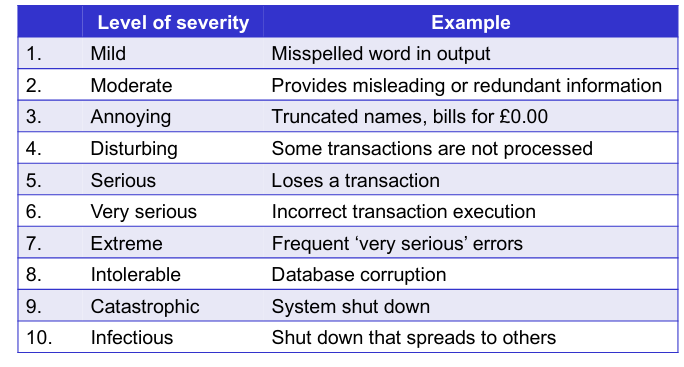
\includegraphics[scale=0.7]{severity}
\end{center}
\section{Implications}
All of these forms of testing are relevant. Since regression testing is almost impossible to avoid, it is worth planning for it.\\
\\
One way to do this is to ensure that, wherever possible, you store test cases (inputs and predicted outputs) in files, for ease of reuse.\\
\\
You should aim to record the outcomes of tests in a systematic matter, adding them to a file or database


\end{document}